\clearpage
\VerdierPhysicalPageAnchor{0139}%
\begingroup
\normalsize
\setlength{\parskip}{0pt}%
\setlength{\emergencystretch}{1.5em}%
\setlength{\abovedisplayskip}{1pt plus 1pt minus 1pt}%
\setlength{\belowdisplayskip}{1pt plus 1pt minus 1pt}%

\VerdierSemanticAnchor{ch2-2-2-6-proof-c-continuation}
\noindent 第二个断言与定理 (2.2.2) 得到。因此尚需证明第二个断言。
\VerdierSemanticAnchor{ch2-2-2-6-proof-b-setup}%
设 $T$ 为 $\mathcal D(S^{-1})$ 中那些同构于 $\mathcal D$ 的特异三角
在 $Q$ 下的像的三角所成的集合。
\VerdierSemanticAnchor{ch2-2-2-6-proof-b-tri-trii}%
不难验证，集合 $T$ 具有性质 TRI 与 TRII。为证明它具有性质 TRIII，
我们需要下述引理：

\VerdierSemanticAnchor{ch2-2-2-7}
\smallskip
\noindent\textbf{引理 2.2.7.}\quad
\begingroup\itshape
设 $u\colon X\longrightarrow Y$ 与 $u'\colon X'\longrightarrow Y'$ 为
$\mathcal D$ 的两个态射，并设

\VerdierSemanticAnchor{ch2-2-2-7-localized-square}
\begin{center}
  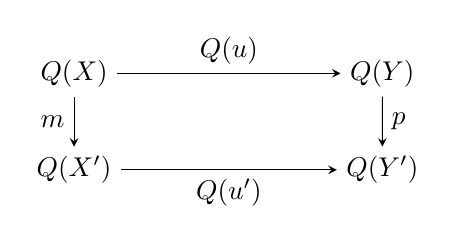
\begin{tikzpicture}[>=stealth,line width=.38pt,x=1.70cm,y=1.25cm,
    scale=.98,transform shape]
    \node (QX)  at (0,1) {$Q(X)$};
    \node (QY)  at (2.35,1) {$Q(Y)$};
    \node (QXp) at (0,0) {$Q(X')$};
    \node (QYp) at (2.35,0) {$Q(Y')$};
    \draw[->] (QX) -- node[above] {$Q(u)$} (QY);
    \draw[->] (QXp) -- node[below] {$Q(u')$} (QYp);
    \draw[->] (QX) -- node[left] {$m$} (QXp);
    \draw[->] (QY) -- node[right] {$p$} (QYp);
  \end{tikzpicture}
\end{center}

\noindent 为 $\mathcal D(S^{-1})$ 中的交换图。
\VerdierSemanticAnchor{ch2-2-2-7-common-representative}%
则存在态射 $u''\colon X''\longrightarrow Y''$，以及 $\mathcal D$ 中的
两个交换图：

\begin{center}
  \VerdierSemanticAnchor{ch2-2-2-7-denominator-square}%
  \begin{tikzpicture}[>=stealth,line width=.38pt,x=1.55cm,y=1.15cm,
    scale=.95,transform shape]
    \node (Xpp) at (0,1) {$X''$};
    \node (Ypp) at (2,1) {$Y''$};
    \node (X)   at (0,0) {$X$};
    \node (Y)   at (2,0) {$Y$};
    \draw[->] (Xpp) -- node[above] {$u''$} (Ypp);
    \draw[->] (X) -- node[below] {$u$} (Y);
    \draw[->] (Xpp) -- node[left] {$s$} (X);
    \draw[->] (Ypp) -- node[right] {$t$} (Y);
    \node at (3.25,.50) {$s,t\in S$};
    \node at (4.50,0) {$,$};
  \end{tikzpicture}
  \par\smallskip
  \VerdierSemanticAnchor{ch2-2-2-7-numerator-square}%
  \begin{tikzpicture}[>=stealth,line width=.38pt,x=1.55cm,y=1.15cm,
    scale=.95,transform shape]
    \node (Xpp) at (0,1) {$X''$};
    \node (Ypp) at (2,1) {$Y''$};
    \node (Xp)  at (0,0) {$X'$};
    \node (Yp)  at (2,0) {$Y'$};
    \draw[->] (Xpp) -- node[above] {$u''$} (Ypp);
    \draw[->] (Xp) -- node[below] {$u'$} (Yp);
    \draw[->] (Xpp) -- node[left] {$f$} (Xp);
    \draw[->] (Ypp) -- node[right] {$g$} (Yp);
    \node at (3.10,0) {$,$};
  \end{tikzpicture}
\end{center}

\VerdierSemanticAnchor{ch2-2-2-7-fraction-identities}
\noindent 使得 $m=Q(f)Q(s)^{-1}$ 且 $p=Q(g)Q(t)^{-1}$。
\endgroup

\VerdierSemanticAnchor{ch2-2-2-6-proof-b-triii-reduction}
\par\noindent 暂且承认该引理，并证明集合 $T$ 具有性质 TRIII。利用
集合 $T$ 的定义，问题归结为证明如下断言：给定 $\mathcal D$ 的两个
特异三角：

\VerdierSemanticAnchor{ch2-2-2-6-proof-b-distinguished-triangles}
\[
  (X,Y,Z,u,v,w)\,,\qquad
  (X',Y',Z',u',v',w')
\]

\noindent 以及 $\mathcal D(S^{-1})$ 中的交换图：

\VerdierSemanticAnchor{ch2-2-2-6-proof-b-localized-square}
\begin{center}
  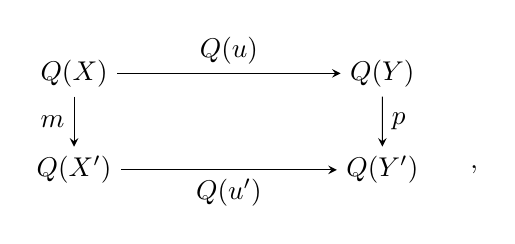
\begin{tikzpicture}[>=stealth,line width=.38pt,x=1.70cm,y=1.25cm,
    scale=.98,transform shape]
    \node (QX)  at (0,1) {$Q(X)$};
    \node (QY)  at (2.35,1) {$Q(Y)$};
    \node (QXp) at (0,0) {$Q(X')$};
    \node (QYp) at (2.35,0) {$Q(Y')$};
    \draw[->] (QX) -- node[above] {$Q(u)$} (QY);
    \draw[->] (QXp) -- node[below] {$Q(u')$} (QYp);
    \draw[->] (QX) -- node[left] {$m$} (QXp);
    \draw[->] (QY) -- node[right] {$p$} (QYp);
    \node at (3.05,0) {$,$};
  \end{tikzpicture}
\end{center}

\VerdierSemanticAnchor{ch2-2-2-6-proof-b-p140-boundary}
\VerdierSemanticAnchor{ch2-2-2-6-p140-boundary}
\endgroup
